\section{Auswertung}
\label{sec:Auswertung}
\subsection{Messung des magnetischen Dipols mithilfe der Gravitation}
Mithilfe der Formel \eqref{eq:grav_dip} und \eqref{eq:bfeld} erhält man folgende, nurnoch von den Messgrößen abhängige, Formel:
\begin{equation}
    \mu_\text{Dipol} = \frac{r}{I}\frac{mg\left(R^2+x^2\right)^{3/2}}{N\mu_0R^2}
\end{equation}
Wobei gilt $x=\SI{6.9}{\centi\meter}$, $R=\SI{10.9}{\centi\meter}$, $m=\SI{1.4}{\gram}$ und $N=\num{195}$.
Es folgen die gemessenen Werte zusammen mit dem jeweilig entsprechenen Dipolmoment:
%
\begin{table}[H]
\label{tab:gravtab}
    \centering
    \caption{Messungen des Graviatationsaufbaus.}
    \begin{tabular}{S[table-format=2.1(0)e0] S[table-format=1.2(0)e0] S[table-format=1.3(0)e0] }
        \toprule
        {$r/\si{\centi\meter}$} & {$I/\si{\ampere}$} & {$\mu_\text{Dipol}/\si{\ampere\meter\squared}$} \\
        \midrule
        6.0     & 1.7   & 0.357    \\
        6.5     & 1.8   & 0.366    \\
        7.0     & 1.95  & 0.364    \\
        7.5     & 2.05  & 0.371    \\
        8.0     & 2.15  & 0.377    \\
        8.5     & 2.25  & 0.383    \\
        9.0     & 2.4   & 0.380    \\
        9.5     & 2.5   & 0.385    \\
        10.0    & 2.6   & 0.390    \\
        10.5    & 2.75  & 0.387    \\
        \bottomrule
    \end{tabular}
\end{table}
In der Abbildung \ref{fig:grav} sind die Messwerte aufgetragen und eine lineare Ausgleichsgerade ist durch diese gezogen.
\begin{figure}[H]
  \centering
  \includegraphics{build/praez.pdf}
  \caption{.}
  \label{fig:grav}
\end{figure}
Damit folgt eine Steigung von $m=0.0312\pm 0.005\si{\tesla\per\meter}$
\noindent Es resultiert ein Wert von
\begin{equation*}
\mu_\text{Dipol} = \SI{0.447\pm0.018}{\ampere\meter\squared}
\end{equation*}
für das magnetische Dipolmoment.
Der Fehler wurde hier nach der Gaußschen Fehlerfortpflanzung berechnet:
\begin{equation*}
  \symup{\Delta} \mu_{Dipol} = \sqrt{(\symup{\Delta} m\frac{m_g \cdot g}{m^2})^2}
\end{equation*}

%
\subsection{Bestimmung des magnetischen Moments die Schwingungsdauer}
Die für die Messung erhaltenen Werte befinden sich in Tabelle \ref{tab:schwing}.
\begin{table}[H]
    \centering
    \caption{Messwerte der Schwingung}
    \label{tab:schwing}
    \begin{tabular}{S[table-format=1.2(0)e0] S[table-format=2.2(0)e0] S[table-format=4.3(0)e0] S[table-format=1.3(0)e0] }
        \toprule
        {$I/\si{\ampere}$} & {$T/\SI{e-1}{\second}$} & {$\frac{1}{B}/\si[per-mode=reciprocal]{\per\tesla}$} & {$T^2/\si{\second\squared}$}\\
        \midrule
        0.50   & 19.84  & 1481.481  & 3.936\\
        1.00   & 14.68  &  740.741  & 2.155\\
        1.25   & 14.66  &  592.592  & 2.149\\
        1.50   & 12.12  &  493.827  & 1.468\\
        2.00   & 11.65  &  370.370  & 1.357\\
        2.50   & 10.37  &  296.296  & 1.075\\
        3.00   &  9.50  &  246.913  & 0.902\\
        3.25   &  9.03  &  227.920  & 0.815\\
        3.50   &  8.78  &  211.640  & 0.771\\
        4.00   &  8.25  &  185.185  & 0.681\\
        \bottomrule
    \end{tabular}
\end{table}
\noindent $T^2$ wird in Abbildung gegen $1/B$ aufgetragen.
Durch dieses Werte wird eine Gerade mittels linearer Regression aufgetragen.
\begin{figure}[H]
  \centering
  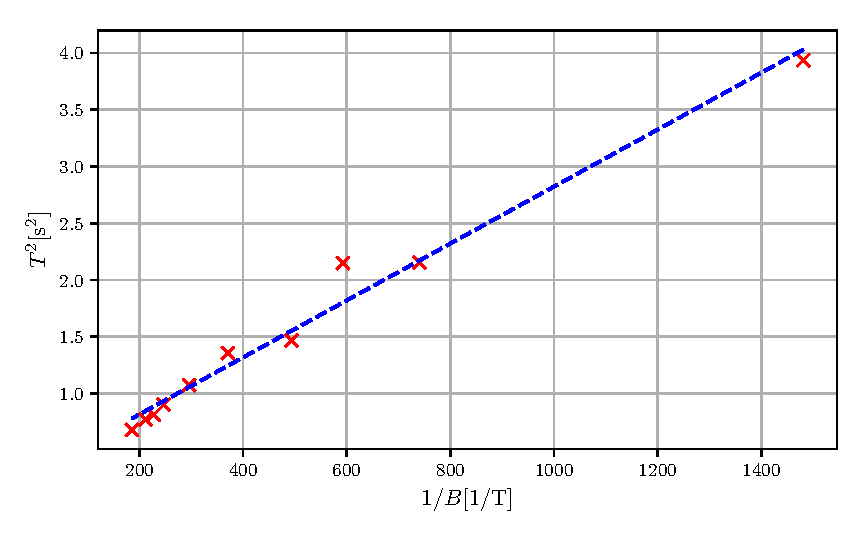
\includegraphics{build/schwing.pdf}
  \caption{.}
  \label{fig:schwing}
\end{figure}
\noindent Daraus folgt eine Steigung von $m=\SI{2.51 \pm 0.12e-3}{\second\squared\tesla}$ für die lineare Ausgleichsgerade.
Das magnetische Moment lässt sich dann nach Formel \eqref{eq:schwing} berechnen:
\begin{equation}
  \mu_\text{Dipol}= \frac{4\cdot \pi^2 \cdot J}{m}=\SI{0.64 \pm 0.304}{\ampere\meter\squared}
\end{equation}
Der Fehler wurde hier mit der Gaußschen Fortpflanzung nach
\begin{equation*}
  \symup{\Delta} \mu_{Dipol} = \sqrt{(\symup{\Delta} m\frac{4 \pi^2 J}{m^2})^2}
\end{equation*}
%
\subsection{Bestimmung des magnetischen Moments über Präzession}
Da es schwierig ist eine konstante Frequenz einzustellen sind die für die Messung angegebenen Werte gemittelt.
Diese Werte befinden sich in Tabelle \ref{tab:praez}. Die Abweichungen wurden hier über die Streuung des Mittelwertes berechnet.
\begin{equation*}
  \symup{\Delta} T = \sqrt{\frac{1}{N(N-1)}\sum_{i=1}^{N}(T_i-\bar{T})^2}
\end{equation*}
\begin{equation*}
  \symup{\Delta} \nu = \sqrt{\frac{1}{N(N-1)}\sum_{i=1}^{N}(\nu_i-\bar{\nu})^2}
\end{equation*}

\begin{table}
    \centering
    \caption{Messwerte der Präzession}
    \label{tab:praez}
    \begin{tabular}{S[table-format=1.2] S[table-format=2.2(3)] S[table-format=1.2(3)]}
        \toprule
        {$B/\SI{e-3}{\tesla}$} & {$\bar{T}/\si{\second}$} & {$\bar{\nu}/\si{\hertz}$}\\
        \midrule
        0.67   & 29.00\pm 0.41  &  6.97\pm 0.17\\
        1.35   & 18.59\pm 0.84  &  7.56\pm 0.38\\
        2.00   & 10.99\pm 0.59  &  6.60\pm 0.43\\
        2.70   &  8.47\pm 0.16  &  6.53\pm 0.09\\
        3.30   &  6.96\pm 0.25  &  6.70\pm 0.38\\
        3.70   &  6.41\pm 0.17  &  6.93\pm 0.33\\
        4.00   &  6.31\pm 0.26  &  6.36\pm 0.29\\
        4.70   &  5.49\pm 0.34  &  7.36\pm 0.44\\
        5.00   &  4.51\pm 0.21  &  6.60\pm 0.49\\
        5.40   &  4.60\pm 0.18  &  6.90\pm 0.58\\
        \bottomrule
    \end{tabular}
\end{table}
\noindent In der Abbildung \ref{fig:praez} wurde die reziproke Periodendauer gegen die Magnetfeldstärke aufgetragen.
Zusätzlich wurde eine Regressionsgerade aufgetragen.
\begin{figure}[H]
  \centering
  \includegraphics{build/praez.pdf}
  \caption{.}
  \label{fig:praez}
\end{figure}
\noindent Für die Steigung der Geraden ergibt sich ein Wert von $m=\SI[per-mode=reciprocal]{39.5\pm1.7}{\per\second\per\tesla}$.
Damit lässt sich das magnetische Moment nach Gleichung \eqref{eq:praez} berechnen:
\begin{equation}
     \mu_\text{Dipol}=m\cdot 2\pi \cdot L .
\end{equation}
Die Abweichungen der Werte wurden hier mit der Gaußschefehlerfortpflanzung berechnet:
\begin{equation*}
  \symup{\Delta} L = \sqrt{(\symup{\Delta}\nu 2 \pi J)^2 }
\end{equation*}
\begin{equation*}
\symup{\Delta} \mu_\text{Dipol} = \sqrt{(\symup{\Delta} L 2 \pi m)^2 + (\symup{\Delta} m 2\pi L)^2 }
\end{equation*}
\begin{table}[H]
    \centering
    \caption{Drehimpulse und Dipolmomente}
    \label{tab:dipolp}
    \begin{tabular}{S[table-format=1.2(3)] S[table-format=1.3(3)]}
        \toprule
        {$L/\SI{e-3}{\kilogram\meter\squared\per\second}$} & {$\mu_{Dipol}/\si{\ampere\meter\squared}$} \\
        \midrule
        1.78\pm 0.04   & 0.441\pm 0.022\\
        1.93\pm 0.09   & 0.478\pm 0.031\\
        1.69\pm 0.11   & 0.419\pm 0.033\\
        1.67\pm 0.02   & 0.414\pm 0.011\\
        1.71\pm 0.09   & 0.424\pm 0.029\\
        1.77\pm 0.08   & 0.439\pm 0.027\\
        1.63\pm 0.07   & 0.404\pm 0.025\\
        1.88\pm 0.11   & 0.466\pm 0.034\\
        1.69\pm 0.13   & 0.419\pm 0.037\\
        1.76\pm 0.15   & 0.437\pm 0.042\\
        \bottomrule
    \end{tabular}
\end{table}
Daraus ergibt sich im Mittel folgendes Dipolmomnt:
\begin{equation*}
  \bar{\mu}_{Dipol}= 0.4341\pm 0.0291 \si{\ampere\meter\squared} .
\end{equation*}
